\documentclass[10pt,twocolumn,twoside,a4paper]{article} % report

\usepackage[slovak,english]{babel}
\usepackage[IL2]{fontenc}
\usepackage[utf8]{inputenc}
\usepackage{graphicx}
\usepackage{url}
\usepackage{hyperref}

\usepackage{cite}

\graphicspath{ {./images/} }

\pagestyle{headings}

\title{Personalized Recommendation Systems in Social Media\thanks{Semester project for the course Engineering Methods, academic year 2024/25, supervised by Ing. Richard Marko, PhD.}}

\author{Yevhenii Deshchenko\\[2pt]
	{\small Slovak Technical University in Bratislava}\\
	{\small Faculty of Informatics and Information Technology}\\
	{\small \texttt{xdeshchenko@stuba.sk}}
}

\date{\small 14 December 2024}

\begin{document}

\maketitle

\begin{abstract}
With the growing popularity of social media, recommendation systems have become increasingly complex and sophisticated. 
These systems rely on a variety of algorithms, including those based on graph theory, statistics, machine and deep learning. 
Content-based recommendation systems vary significantly across many different social media platforms, as they depend on the 
type of primary content users share and the options provided for user interaction with the content. 
Most approaches use as much data as available, leading to massive data collection that raises multiple concerns, such as privacy issues.


As social media platforms continue to grow in popularity, the inner workings of these algorithms are often kept secret,
as they have become valuable tools for third parties seeking to exploit them for visibility and influence.
This exploitation frequently aims to push content with political or other agendas, in an effort to gain popularity on these platforms.
However, there are exceptions, such as Twitter, which made its recommendation algorithm public after a data breach.
This decision led to significant criticism from its user base. The secrecy and potential for manipulation continue to
spark debates about the role and transparency of recommendation systems in shaping user experiences and content visibility on social media.
\end{abstract}

% 
\includegraphics[width=\textwidth]{fiit.eps}

\section{Introduction} 

In a modern era where social media has become an integral part of daily life, personalized recommendation systems play a
crucial role in enhancing marketing, entertainment, and the overall user experience. By predicting and delivering content
that resonates with users, these systems contribute significantly to social media growth, fostering higher user engagement
and supporting an interconnected ecosystem of content creators, businesses, and users alike.

While these systems are built upon statistical and mathematical foundations, practical implementations vary widely.
They often combine several approaches, including complex algorithms, databases, big data analytics, machine learning,
and deep learning techniques, to optimize predictions and deliver tailored content. 

However, the reliance on extensive user data raises privacy concerns, as large amounts of personal information must
be stored and processed. Additionally, biases within these algorithms can lead to unintended consequences, potentially
skewing recommendations or enabling exploitation. This paper will explore the methodologies behind recommendation systems,
their societal impacts, and the balance between personalization and ethical considerations.

\section{Recommendation Systems Overview} \label{rec_sys_overview}
The primary goal of recommendation systems (RS) is to suggest content, connections, posts, or advertisements that may interest the end user. Social media technology has evolved over time and is now embedded in blogs, forums, and other digital forms, facilitating community building, content sharing, and information exchange~\cite{anandhan2018social}. These systems have become integral in helping users navigate vast amounts of content efficiently, allowing platforms to deliver more personalized experiences.

\subsection{Social Media Overview}
Social media platforms can be classified into several categories~\cite{anandhan2018social} based on their primary function and user interaction patterns:
\begin{itemize}
    \item \textbf{Digital Libraries:} Platforms like Pinterest and Flickr act as digital libraries where users can share, categorize, and access large collections of images, documents, or other resources. Recommendation systems on these platforms focus on content discovery, suggesting relevant media or documents based on specific, determined user preferences.
    \item \textbf{Forums:} Platforms such as Reddit and Stack Overflow allow users to engage in topic-focused discussions and share information. Here, recommendation systems suggest relevant threads, discussions, or posts based on user interactions and interest tags.
    \item \textbf{Blogs:} Platforms like Medium and Tumblr are designed for content creation, where users can write articles, stories, or posts. Recommendation systems on blogs aim to match readers with articles that align with their interests, reading history, and trending topics.
    \item \textbf{Social Networks:} Platforms such as Facebook, Instagram, and Twitter are built around user-to-user connections and content sharing. These platforms rely heavily on recommendation systems to suggest new connections, posts, and advertisements, fostering interaction between content creators, advertisers, and consumers.
    \item \textbf{Other:} Platforms like YouTube blend multiple features from the above categories, creating a multi-functional space that combines video sharing, social networking, and content discovery.
\end{itemize}

One of the most widespread applications of recommendation systems is within social networks such as Facebook, Instagram, and Twitter. These systems play a pivotal role in connecting content creators and advertisers with consumers by suggesting relevant posts, trending topics, or advertisements tailored to user preferences. As users engage with these platforms, recommendation systems analyze behavior, including likes, shares, comments, and search queries, to curate personalized content. This personalization aims to enhance user engagement, increase time spent on the platform, and improve overall user satisfaction.

\subsection{Types of Recommendation Systems}
The algorithms behind personalized recommendation systems are typically classified into content-based filtering and collaborative filtering \cite{raghavendra2018personalized}.

In content-based filtering, the algorithm constructs a profile of the target user, which is then used to determine what items—such as posts or advertisements—would be appropriate to recommend. This approach works by first identifying item characteristics and assigning them keywords and tags. Using machine learning algorithms, decision trees, and clustering techniques, the system recommends items with features similar to those previously liked or positively reviewed by the user~\cite{raghavendra2018personalized}\cite{contentvscollaborative}.

In collaborative filtering, the recommendation system bases its suggestions on user behavior analysis. By comparing patterns and preferences across a large user base, collaborative filtering algorithms identify similarities between users and recommend items that similar users have interacted with.

Another two, less significant approaches would be based on humanistic and social information - it is when system provides recommendations by
analyzing the information provided by users when they register, or knowledge-based, which is providing recommendations based on external knowledge

\section{Data collection and privacy issues} \label{data_issues}
With the growth of use of recommendation systems, new problems arise, such as data collection and privacy issues.
Recommendation systems collect massive arrays of user base of each user, such as gender, location, occupation, search history, likes, views and so on.
There are three \cite{PrivacyProtectionSurvey} main stages in the process of presonalized service that may course users privacy concerns:
\begin{itemize}
    \item \textbf{User Modeling:} User's personal information preferences and need are collected. This data is obtained explicitly, when provided by the user himself or herself, or implicitly, such as tracking user's search history, likes, etc. After that, this dataset should be represented by appropriate data structure of the user model for further processing and calculation. Privacy issues may arise at this stage in impoper access, collection, transmission etc.
    \item \textbf{Calculation:} At this stage calculations are carried out to make later recommendation. Privacy issues here may arise in impoper analysis, merging of data, etc.
    \item \textbf{Result generation:} This is the last stage where recommendation system gets results after calculation. Privacy concerns arising from this stage include impoper analysis, transmission of data, etc.
\end{itemize}

\section{Content manipulation and transparency challenges} \label{content_manipulation}
Recommendation systems are frequently targeted by malicious attacks designed to manipulate the visibility of posts, advertisements, or other information, often to achieve maximum exposure or push specific agendas~\cite{propagandasafety}. Collaborative filtering, when not properly safeguarded, is particularly vulnerable to such attacks~\cite{ManipulationAttacks}. Since most modern recommendation systems employ a hybrid approach combining collaborative and content-based filtering, it is reasonable to conclude that all systems are susceptible to manipulation unless robust countermeasures are implemented by social media platforms.

One of those attacks is manipulation attack. \cite{ManipulationAttacks}. In this scenario, collaborative filtering can be compromised by introducing a substantial number of fake accounts controlled by the attacker. These accounts interact with specific content, influencing the system to recommend it to a broader audience. This raises several concerns, particularly because collaborative filtering is among the most widely adopted and effective recommendation algorithms. Platforms must assess the risk of potential attackers, such as political entities aiming to influence older demographics or authoritarian governments seeking to shape young users' opinions.

% \begin{figure}[h!]
%     \centering
%     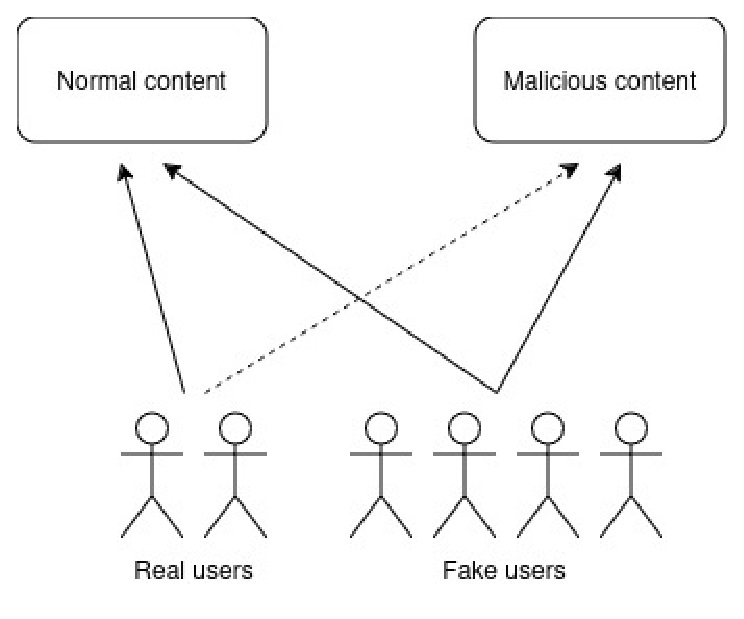
\includegraphics[width=\textwidth]{manipulation.eps}
%     \caption{Diagram showing how recommendation system manipulation works}
%     \label{fig:recommendation_manipulation}
% \end{figure}

% 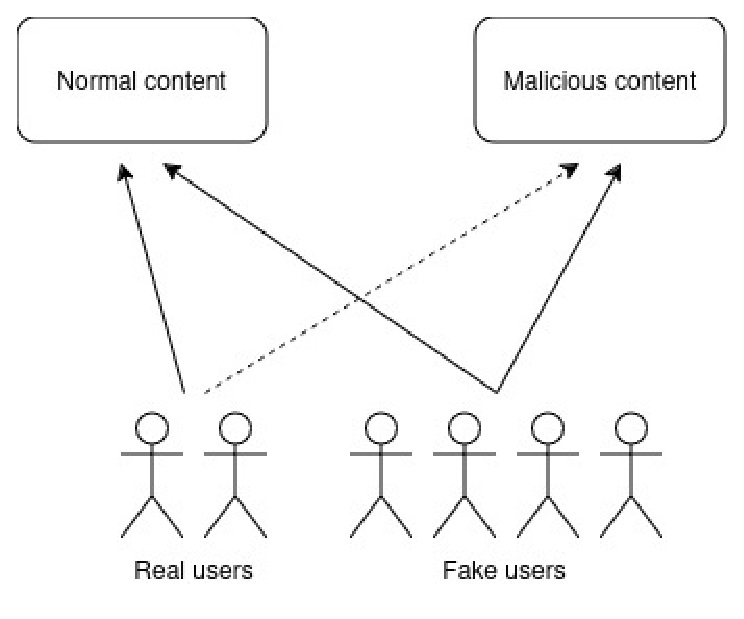
\includegraphics[width=\textwidth]{manipulation.eps}
% 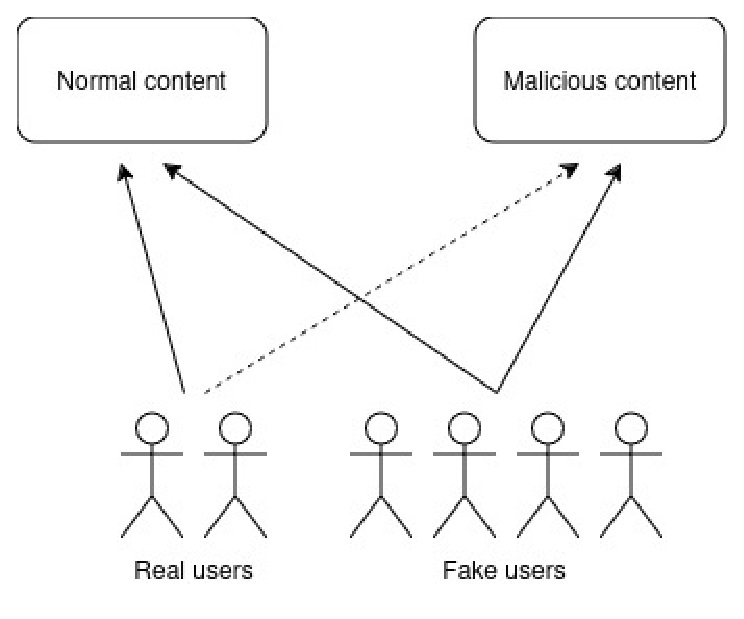
\includegraphics[width=0.8\textwidth]{manipulation.eps}  % 80% of text width
\begin{figure}[h!]
    \centering
    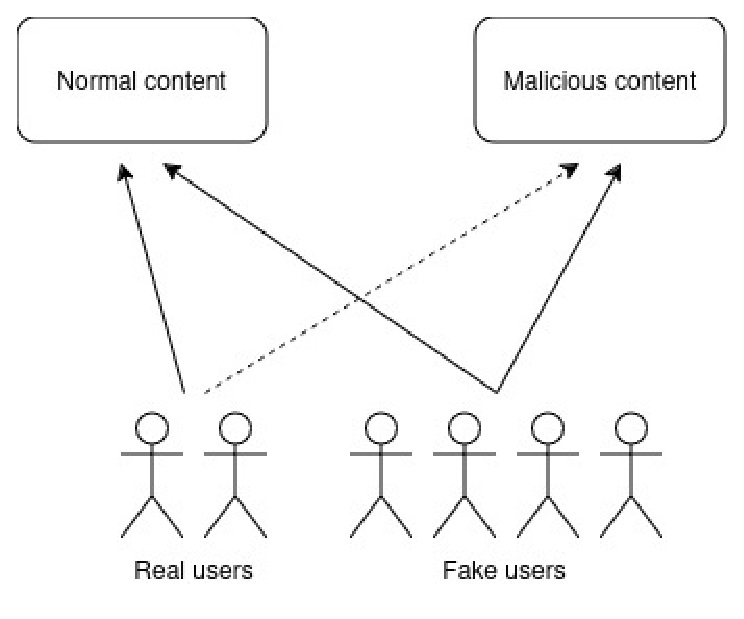
\includegraphics[width=0.4\textwidth, height=0.3\textheight]{manipulation.eps}
    \caption{Diagram showing how recommendation system manipulation works}
    \label{fig:recommendation_manipulation}
\end{figure}

As Figure \ref{fig:recommendation_manipulation} shows, third parties may force certain group of similar users to view certain content, by imitating similarity.

Effective countermeasures \cite{ManipulationAttacks} to mitigate these risks include:

\begin{itemize}
    \item \textbf{Preventing mass account registration.} Collaborative filtering relies on extensive user engagement with specific content to influence recommendations. By implementing strict controls to prevent large-scale fake account creation, platforms can significantly reduce the risk of low-effort campaigns designed to bias the system.
    \item \textbf{Restricting new users influence on recommendations.} Although it is challenging to identify malicious intent at the registration stage, limiting the initial impact of new users on the recommendation system can mitigate potential biases. This approach ensures that even if fake accounts are created, their effect on recommendations remains minimal.
    \item \textbf{Limiting the influence of low-activity users.} Fake accounts are often characterized by minimal activity. Social media platforms can prioritize input from highly active users while de-emphasizing contributions from less active ones. While this may disadvantage legitimate low-activity users, it enhances the system's overall robustness against manipulation.
    \item \textbf{Detecting suspicious behavior.} Fake accounts typically exhibit behavioral patterns that differ from those of genuine users. Platforms can employ machine learning techniques to identify and flag anomalies, such as automated activity or coordinated actions, to detect and neutralize these accounts proactively.
\end{itemize}

\subsection{Practical approaches}
There are multiple approaches used in the modern social media platform to secure their space and ultimately recommendation systems from third-party influences.
To prevent masses of fake accounts flooding into the platform, developers typically make registration requirements. Such requirements could be
\begin{itemize}
    \item \textbf{Temporary email address restriction.} Platforms may ban certain email providers so that users have to have legitimate email addresses. If on the platform every user should have unique email address, it will make slight problems for the malicious parties, but not significant, as they could, theoretically, create their own mail server which will not be in the ban list of the social media platform.
    \item \textbf{Phone number confirmation.} This is, by far, one of the most effective countermeasures against mass fake registration. The reason is, comparing to the email addresses, that acquiring such amount of phone numbers is a relatively challanging task.
    \item \textbf{CAPTCHA.} CAPTCHA is acronim, which stands for Completely Automated Public Turing test to tell Computers and Humans Apart. \cite{singh2014survey} CAPTCHA presents new user with a certain task, which is trivial to a human being, but too complicated to be solved by automated scripts. The tasks could be text-based, image-based or invisible.
\end{itemize}

To detect suspicious behavour, social media platforms use an array of techniques. Accounts which produced suspicious activity, depending on software implementation, company policy and situation, either get a ban, or get challanged with a CAPTCHA, to verify if it is a real human.

\subsection{Using CAPTCHA against registered fake accounts}
Besides phone number confirmation, CAPTCHA remains one of the most crucial methods and actively used by social media platforms.

There are three main properties \cite{singh2014survey} CAPTCHA must satisfy
\begin{itemize}
    \item CAPTCHAs must be easily solvable for humans, otherwise they are messing up app usage
    \item It should be an automated proccess, machine must generate tasks and in the same automated way grade answers
    \item It must be hard for another automated system to solve, not knowing generation algorithm
\end{itemize}

Table~\ref{tab:captcha_types} illustrates various types of CAPTCHA and their respective features and drawbacks~\cite{singh2014survey}.
Text-based CAPTCHAs are the simplest and most widely used, but they are vulnerable to Optical Character Recognition (OCR) techniques, which bots can exploit.
Image-based CAPTCHAs add a layer of difficulty by requiring users to identify objects or patterns,
yet they pose accessibility challenges for visually impaired users.
Similarly, audio-based CAPTCHAs are designed for such users but require a good understanding of spoken language,
which can create difficulties due to similar-sounding characters.
Video-based CAPTCHAs, though highly secure, require significant bandwidth and can be cumbersome to download.
Puzzle-based CAPTCHAs challenge users with time-intensive tasks and are less commonly employed due to their complexity~\cite{singh2014survey}.

\begin{table*}[t] \label{tab:captcha_comparison}
    \centering
    \caption{Comparison of Different CAPTCHA Types}
    \begin{tabular}{|l|p{0.35\textwidth}|p{0.35\textwidth}|}
    \hline
    \textbf{Type of CAPTCHA} & \textbf{Features} & \textbf{Drawbacks} \\ \hline
    Text-Based & Simple to implement, widely used & Can be solved by OCR, may confuse users due to distortion \\ \hline
    Image-Based & Requires identifying objects or patterns & Not user-friendly for visually impaired users \\ \hline
    Audio-Based & Designed for visually impaired users & Requires good understanding of spoken language, similar sounds can confuse \\ \hline
    Video-Based & Uses dynamic visual content for challenges & Requires high bandwidth, difficult to download \\ \hline
    Puzzle-Based & Users solve puzzles to pass & Time-consuming, challenging for users unfamiliar with puzzles \\ \hline
    \end{tabular}
    \label{tab:captcha_types}
\end{table*}

Despite their effectiveness, CAPTCHAs are not foolproof.
Advances in artificial intelligence have enabled bots to bypass traditional CAPTCHAs, particularly text-based systems.
To counter this, social media platforms are adopting newer approaches, such as behavior-based CAPTCHA systems like reCAPTCHA v3,
which analyze user interactions to distinguish humans from bots without requiring explicit challenges.
The ongoing evolution of CAPTCHA systems highlights the need for continuous innovation to stay ahead of increasingly sophisticated bot technologies.
As security demands grow, the integration of adaptive techniques and multi-layered approaches remains critical in preserving the integrity of
user registration processes and online interactions.

\section{Future challanges in recommendation systems} \label{future_challanges}

\section{Conclusion} \label{conclusion}
The evolution of personalized recommendation systems has transformed social media, enabling platforms to deliver more relevant and engaging content to users. By leveraging sophisticated algorithms, machine learning, and big data analytics, these systems are able to predict user preferences and deliver tailored experiences that increase platform engagement and satisfaction. However, this innovation comes with significant challenges, particularly in the realms of data privacy and content manipulation. As recommendation systems grow in complexity, concerns about user privacy, ethical implications, and transparency continue to mount. 

The societal impact of these systems is profound, influencing not only individual user experiences but also public opinion, trends, and information dissemination. Striking a balance between personalization and ethical responsibility will be crucial for the future of social media. To foster trust and maintain user autonomy, platforms must adopt transparent policies, ensure robust privacy protections, and address potential biases within their recommendation algorithms. As technology advances, ongoing research and open discourse on the ethical dimensions of recommendation systems will be essential in shaping a socially responsible digital ecosystem.

\nocite{*}
\bibliography{literatura}
\bibliographystyle{plain}
\end{document}
